\sisetup{locale = EN} 
\title{\textbf{\rmfamily Discussion of Results}}
\author[~\PersonDiscusion~]{{\PersonDiscusion}}
\institute[\WorkGroup]{ \University}
\date{\dateMC}

%%%%%%%%%%%%%%%%%%%%%%%%%%%%%%%%%%%%%%%%%%%%%%%%%%%%%%%%%%%%%%%%%%%%%%%%%%%%%%%%%%%%%%%%%%%%%%
%   Options for the footline
%%%%%%%%%%%%%%%%%%%%%%%%%%%%%%%%%%%%%%%%%%%%%%%%%%%%%%%%%%%%%%%%%%%%%%%%%%%%%%%%%%%%%%%%%%%%%%
\setbeamertemplate{footline}
{
\leavevmode%
\hbox{%
\begin{beamercolorbox}[wd=0.5\paperwidth,ht=2.25ex,dp=1ex,center]{author in foot}%
\usebeamerfont{author in foot} \parbox{0.5\paperwidth}{\insertsubsection{}}
\end{beamercolorbox}%
\begin{beamercolorbox}[wd=0.11\paperwidth,ht=2.25ex,dp=1ex,center]{title in head/foot}%
\usebeamerfont{title in head/foot}
\end{beamercolorbox}%
\begin{beamercolorbox}[wd=0.385\paperwidth,ht=2.25ex,dp=1ex,right]{date in head/foot}%
\usebeamerfont{date in head/foot}\insertsection{}\hfill
|~Folie \insertframenumber{} \hspace*{2ex}%/ \inserttotalframenumber\hspace*{2ex}
\end{beamercolorbox}}%
\vskip0pt%
}

%%%%%%%%%%%%%%%%%%%%%%%%%%%%%%%%%%%%%%%%%%%%%%%%%%%%%%%%%%%%%%%%%%%%%%%%%%%%%%%%%%%%%%%%%%%%%%
% Options for the timetable
%%%%%%%%%%%%%%%%%%%%%%%%%%%%%%%%%%%%%%%%%%%%%%%%%%%%%%%%%%%%%%%%%%%%%%%%%%%%%%%%%%%%%%%%%%%%%%

% \makeatletter
% \newcommand{\setcurrtime}[1]{%
%   \set@time\curr@hour\curr@mins#1\@nil
% }
% \def\set@time#1#2#3:#4\@nil{%
%   \def#1{#3}\def#2{#4}%
% }
% \newcommand{\currtime}[1][00:00]{%
%   \begingroup
%   \set@time\new@hour\new@mins#1\@nil
%   \count\z@=\curr@mins\relax
%   \count\tw@=\curr@hour\relax
%   \advance\count\z@\new@mins\relax
%   \advance\count\tw@\new@hour\relax
%   \ifnum\count\z@>59
%     \advance\count\z@-60
%     \advance\count\tw@\@ne
%   \fi
%   % we have to use \count\z@ and \count\tw@ before
%   % ending the group and printing the result
%   \edef\x{\endgroup\two@digits{\count\tw@}:\two@digits{\count\z@}}\x
% }
% \makeatother


\begin{document}\selectlanguage{english}
%%%%%%%%%%%%%%%%%%%%%%%%%%%%%%%%%%%%%%%%%%%%%%%%%%%%%%%%%%%%%%%%%%%%%%%%%%%%%%%%%%%%%%%%%%%%%%
\begin{frame}[plain]
\begin{center}
    \begin{tabular}{ccc}
 \parbox{0.33\textwidth}{\LogoInsitute}    &
 ~~~~\parbox{0.33\textwidth}{
\includegraphics[height=1cm]{Logos And Group/LHCb_Logo.png}}   &  \parbox{0.33\textwidth}{\LogoUniversity}\\
\end{tabular}
\end{center}

\maketitle
\end{frame}
%%%%%%%%%%%%%%%%%%%%%%%%%%%%%%%%%%%%%%%%%%%%%%%%%%%%%%%%%%%%%%%%%%%%%%%%%%%%%%%%%%%%%%%%%%%%%%
\section{Discussion of Results}
%%%%%%%%%%%%%%%%%%%%%%%%%%%%%%%%%%%%%%%%%%%%%%%%%%%%%%%%%%%%%%%%%%%%%%%%%%%%%%%%%%%%%%%%%%%%%%
% \begin{frame}{Eure Ergebnisse}
% \begin{itemize}

% \ttfamily
%     \item please help us
%     \item Wir sollten darüber sprechen ob und wie wir Ergebnisse (sinnvoll) sichern. 
% \end{itemize}
% \end{frame}
%%%%%%%%%%%%%%%%%%%%%%%%%%%%%%%%%%%%%%%%%%%%%%%%%%%%%%%%%%%%%%%%%%%%%%%%%%%%%%%%%%%%%%%%%%%%%%
\begin{frame}{Interpret your Results!}

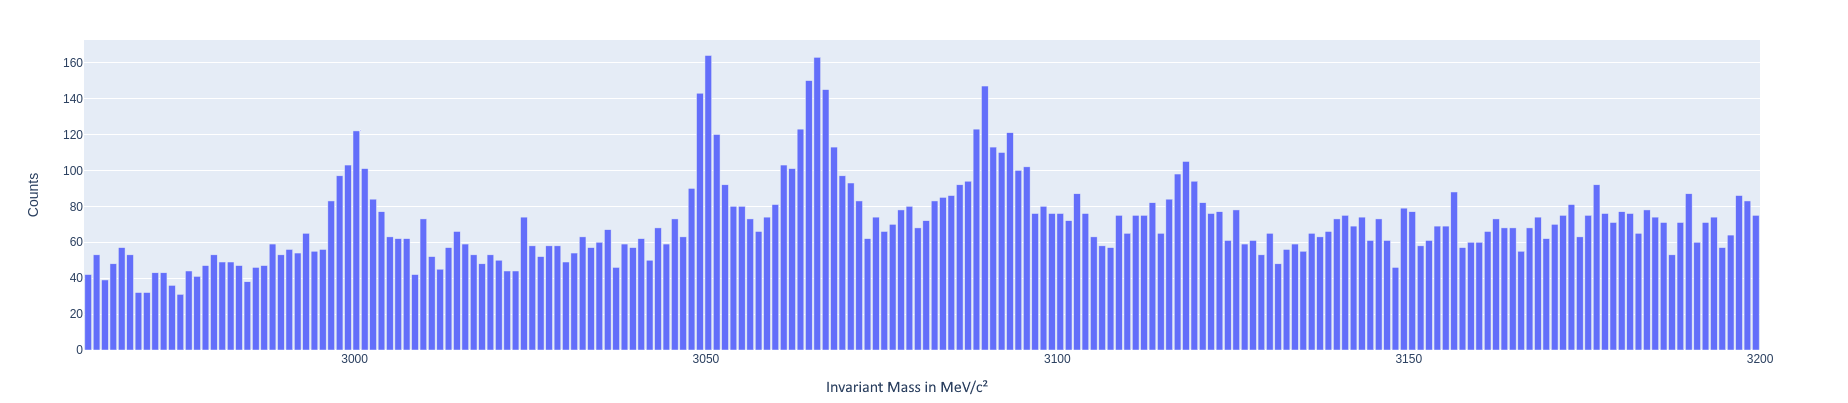
\includegraphics[width=\textwidth]{Figures Discussion/Result_OmegaC.png}

\\ 
\begin{center}
  \Large  $\mathbf{ \Omega_c^0 \rightarrow \Xi_c^+\,K^-}$
\end{center}



   \begin{center} What do you think your results mean? \end{center}

\end{frame}
%%%%%%%%%%%%%%%%%%%%%%%%%%%%%%%%%%%%%%%%%%%%%%%%%%%%%%%%%%%%%%%%%%%%%%%%%%%%%%%%%%%%%%%%%%%%%%
\begin{frame}{Interpret your Results!}
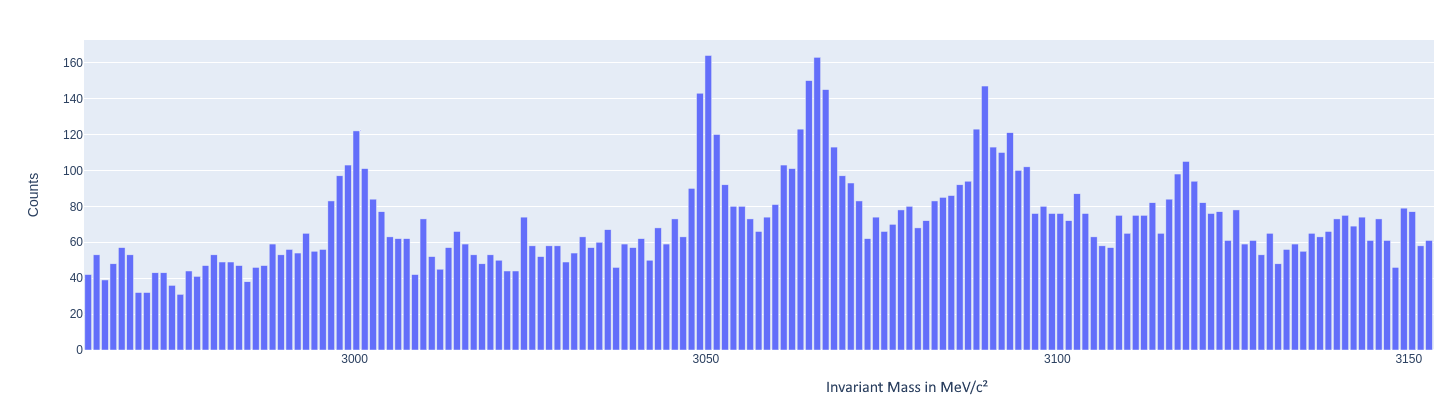
\includegraphics[width=\textwidth]{Figures Discussion/Result_OmegaC_cutted.png}
You can see \textbf{five resonances} at \\ 
\begin{minipage}{0.4\textwidth}
\begin{itemize}
\item $m_1=3000$\,MeV/$c^2$ 
\item $m_2=3050$\,MeV/$c^2$
\item $m_3=3060$\,MeV/$c^2$
\item $m_4=3090$\,MeV/$c^2$
\item $m_5=3119$\,MeV/$c^2$
\end{itemize}\end{minipage}\pause
\begin{minipage}{0.4\textwidth}
\begin{overpic}[width=.9\textwidth,,tics=10]{Figures Lecture on Hadrons/ccBar_spectrum.png}
\put(40,-5){\scriptsize E$_\gamma$ in MeV}
\put(-2,35){\scriptsize \rotatebox[]{90}{Counts}}
\end{overpic}
\end{minipage}
\begin{minipage}{.19\textwidth}
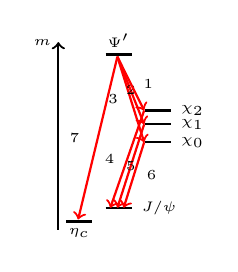
\begin{tikzpicture}[xscale=1,yscale=0.53]
{\fontsize{4}{5} \selectfont
      \draw[thick] (0,0) --++ (0.33,0) node[midway, below] {$\eta_c$};
      \draw[thick] (0.5,0.33) --++ (0.33,0) node[right=1pt] {$J/\psi$};
     \draw[thick] (1,1.9) --++ (0.33,0) node[right=1pt] {$\chi_0$}; 
      \draw[thick] (1,2.33) --++ (0.33,0) node[right=1pt] {$\chi_1$};
      \draw[thick] (1,2.66) --++ (0.33,0) node[right=1pt] {$\chi_2$};
      \draw[thick] (0.5,4) --++ (0.33,0) node[above,midway] {$\Psi'$};
   
    \draw[->,thick,red] (0.65,3.95) -> (0.1515,0.05) node[midway,black,left=4pt] {7};
    \draw[->,thick,red] (0.65,3.95) -> (0.99,1.9) node[midway,black,left=2pt] {3};
    \draw[->,thick,red] (0.65,3.95) -> (0.99,2.33) node[midway,black] {2};
    \draw[->,thick,red] (0.65,3.95) -> (0.99,2.66) node[midway,black,right=2pt] {1};

    \draw[->,thick,red] (0.99,1.9) -> (0.73,0.33) node[midway,black,right=2pt] {6};
     \draw[->,thick,red] (0.99,2.33) -> (0.65,0.33) node[midway,black] {5};
      \draw[->,thick,red] (0.99,2.66) -> (0.56,0.33) node[midway,black,left=2pt] {4};

      
     \draw[->,thick] (-0.1,-0.2) --++ (0,4.5) node[left] {$m$};  
}
   % \draw[<-,thick,blue!90!black] (0.2,0) --++ (0,3.5) node[above=40pt,right,midway,scale=0.8] {$E=h\cdot f_3$};
   % \draw[<-,thick,green!90!blue] (0.4,0) --++ (0,3) node[above=27pt,right,midway,scale=0.8] {$E=h\cdot f_2$};
   % \draw[<-,thick,red] (0.6,0) --++ (0,2) node[right,midway,scale=0.8] {$E=h\cdot f_1$};

    
\end{tikzpicture}
\begin{center}
\tiny{Comparison spectrum of $c\Bar{c}$}
\end{center}
\end{minipage}
\end{frame}
%%%%%%%%%%%%%%%%%%%%%%%%%%%%%%%%%%%%%%%%%%%%%%%%%%%%%%%%%%%%%%%%%%%%%%%%%%%%%%%%%%%%%%%%%%%%%%
\begin{frame}{What do we Learn from this?}
\begin{center}
\begin{itemize}
\begin{spacing}{2}
     \item[]<1-> Which of you can explain the five $\Omega_c^0$ resonances?
    \item[]<2-> \LARGE{We don't know either!}
    \item[]<2-> This is a hot topic!
\end{spacing}
   
   
\end{itemize}    
\end{center}
\end{frame}
%%%%%%%%%%%%%%%%%%%%%%%%%%%%%%%%%%%%%%%%%%%%%%%%%%%%%%%%%%%%%%%%%%%%%%%%%%%%%%%%%%%%%%%%%%%%%%
\subsection{LHCb, 2017}
\begin{frame}{Results LHCb}
 \begin{minipage}{0.49\textwidth}
 \begin{itemize}
        \item<1-> Result of the scientists at the LHCb \hspace{2cm }\ding{220}
        \item<1-> Similar to your results!
    \end{itemize}

\end{minipage}\begin{minipage}{0.49\textwidth}

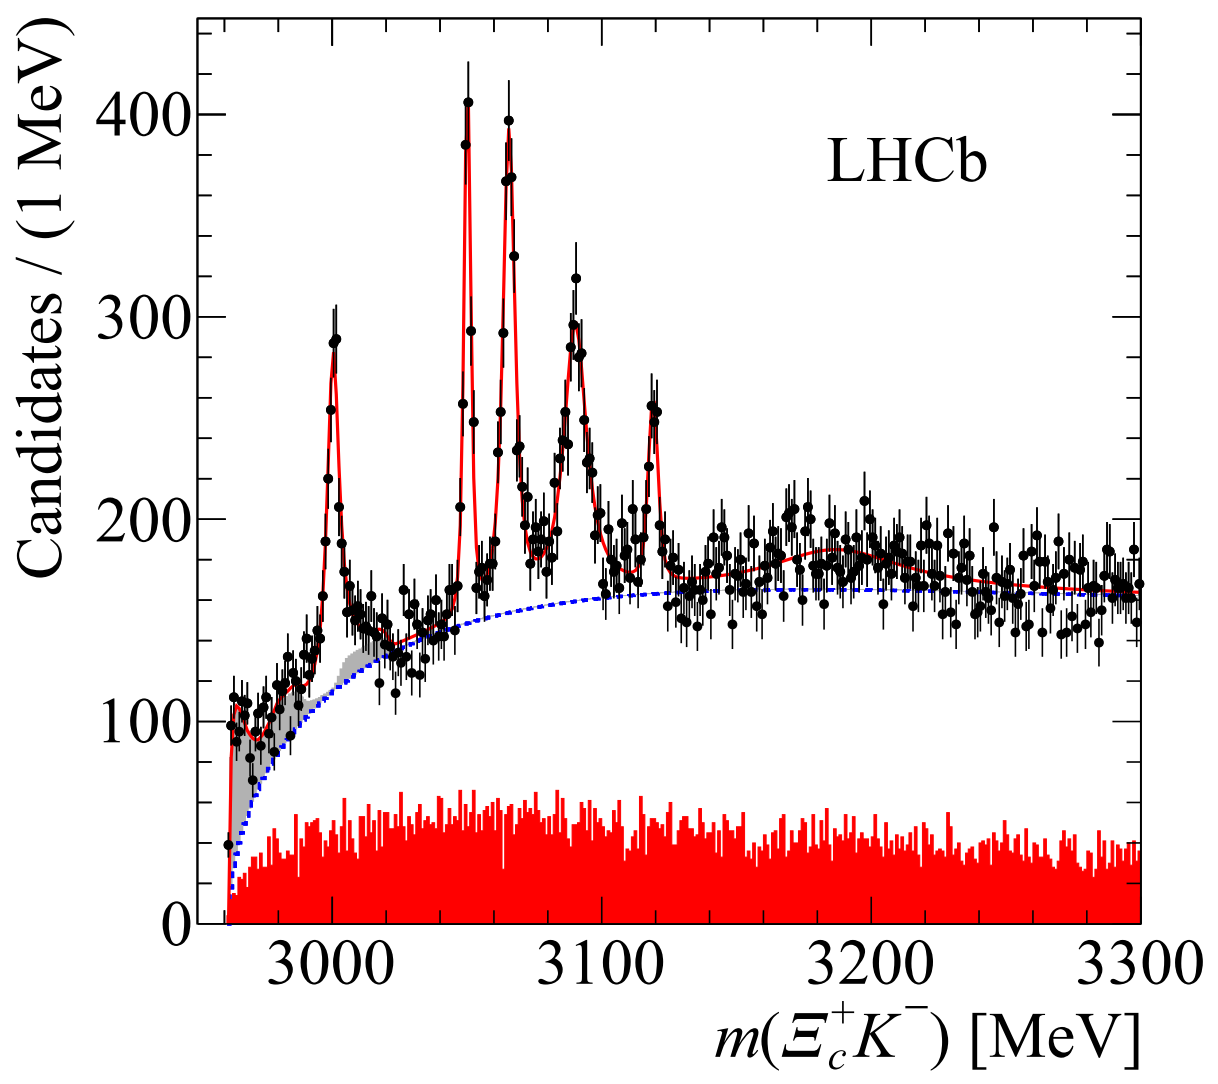
\includegraphics[width=\textwidth]{Figures Discussion/Result_OmegaC_spectrum_LHCb.png}
\end{minipage}

\begin{center}
   \texttt{AND NOW? What does the result tell us?} \\ 
       \ding{43} There are generally many unanswered questions in physics! 
\end{center}
    
\end{frame}
\subsection{}
\begin{frame}

\textbf{\textcolor{red}{Open Questions in Physics}}
    \begin{itemize}
         \item [\ding{73}] Origin of mass: Higgs mechanism
            \item [\ding{73}] Why and how do quarks group into hadrons? There are hadrons with more than three quarks!
            \item [\ding{73}] Why is there more particle matter than antiparticles/antimatter in the universe?
            \item [\ding{73}] Dark matter, dark energy: Are there still \emph{new}, undiscovered particles, forces and physics?
    \end{itemize}

\end{frame}
%%%%%%%%%%%%%%%%%%%%%%%%%%%%%%%%%%%%%%%%%%%%%%%%%%%%%%%%%%%%%%%%%%%%%%%%%%%%%%%%%%%%%%%%%%%%%%
\begin{frame}{The LHCb Collaboration and CERN are Trying to Find Out!}
\begin{minipage}{0.21\textwidth} \begin{center}

\includegraphics[width=0.85\textwidth]{Logos And Group/CERN_logo.png} \\ \vspace{.75cm}

\includegraphics[width=0.85\textwidth]{Logos And Group/LHCb_Logo.png} \\ \vspace{.75cm}
\LogoInsitute
\end{center}\end{minipage}\begin{minipage}{0.82\textwidth}
\textbf{\textcolor{red}{LHCb:} lhcb.web.cern.ch/}
\begin{itemize}
\item 1400 scientists, in front of you are \NumPeople!
\item 86 universities/research centres
\item 18 countries
\vspace{0.5cm}
\end{itemize}\textcolor{red}{\WorkGroup:}\begin{itemize}
    
\item To the website of our group
\item[] \textbf{\WorkGroupWebsite}
\end{itemize}
\end{minipage}

\end{frame}
%%%%%%%%%%%%%%%%%%%%%%%%%%%%%%%%%%%%%%%%%%%%%%%%%%%%%%%%%%%%%%%%%%%%%%%%%%%%%%%%%%%%%%%%%%%%%%

\begin{frame}{Conclusion}
    \begin{itemize}
        \item \textbf{You} have discovered five new particles today!
        \item \textbf{You} learnt today how particle physicists search for new particles.
        \item \textbf{You} got excited about studying physics today :p
        \vspace{0.5cm}
        \item[] Questions about studying, science, physics and more? 
        \begin{itemize}
            \item[\ding{43}] We are still here!
        \end{itemize}
    \end{itemize}
\end{frame}
%%%%%%%%%%%%%%%%%%%%%%%%%%%%%%%%%%%%%%%%%%%%%%%%%%%%%%%%%%%%%%%%%%%%%%%%%%%%%%%%%%%%%%%%%%%%%%
\begin{frame}
\begin{center}
\Huge{Thank you}\normalsize, \\
 for letting us spend the day with you :D
\end{center}
\end{frame}
%%%%%%%%%%%%%%%%%%%%%%%%%%%%%%%%%%%%%%%%%%%%%%%%%%%%%%%%%%%%%%%%%%%%%%%%%%%%%%%%%%%%%%%%%%%%%%
\begin{frame}{References}
    \begin{itemize}\footnotesize
        \item [-] The LHCb Collaboration. Observation of five new narrow $\Omega_c^0$ states decaying to $\Xi_c^+$. In: American Physical Society 118.18 (2017).
    \end{itemize}
\end{frame}
\end{document}